\documentclass{article}
\usepackage{iclr2024_conference,times}

\usepackage[utf8]{inputenc} % allow utf-8 input
\usepackage[T1]{fontenc}    % use 8-bit T1 fonts
\usepackage{hyperref}       % hyperlinks
\usepackage{url}            % simple URL typesetting
\usepackage{booktabs}       % professional-quality tables
\usepackage{amsfonts}       % blackboard math symbols
\usepackage{nicefrac}       % compact symbols for 1/2, etc.
\usepackage{microtype}      % microtypography
\usepackage{xcolor}         % colors
\usepackage{wrapfig}
\usepackage{caption}
\usepackage{subcaption}

\usepackage{mymathstyle} % math style with a bunch of commands defined

\usepackage{cleveref}
\usepackage{algorithm2e}
\usepackage{graphicx}
\crefname{algocf}{alg.}{algs.}
\Crefname{algocf}{Algorithm}{Algorithms}
\RestyleAlgo{ruled}

\usepackage{tikz}
\usetikzlibrary{positioning}
\pgfmathtruncatemacro\distance{1}
\usepackage{fp}

\usepackage{mathrsfs}
\RequirePackage{hypernat}
\usepackage{graphicx}
\usepackage{verbatim}

%region custom commands
\newcommand{\softreliprod}[3]{\left\langle #1, #2 \, \vert \, #3 \right\rangle_\mathrm{rel}}
\newcommand{\reliprod}[2]{\left\langle #1, #2 \right\rangle_\mathrm{rel}}
%endregion


\title{Relational Convolution Networks: A framework for learning compositional relations}

% The \author macro works with any number of authors. There are two commands
% used to separate the names and addresses of multiple authors: \And and \AND.
%
% Using \And between authors leaves it to LaTeX to determine where to break the
% lines. Using \AND forces a line break at that point. So, if LaTeX puts 3 of 4
% authors names on the first line, and the last on the second line, try using
% \AND instead of \And before the third author name.

\author{Antiquus S.~Hippocampus, Natalia Cerebro \& Amelie P. Amygdale \thanks{ Use footnote for providing further information
about author (webpage, alternative address)---\emph{not} for acknowledging
funding agencies.  Funding acknowledgements go at the end of the paper.} \\
Department of Computer Science\\
Cranberry-Lemon University\\
Pittsburgh, PA 15213, USA \\
\texttt{\{hippo,brain,jen\}@cs.cranberry-lemon.edu} \\
\And
Ji Q. Ren \& Yevgeny LeNet \\
Department of Computational Neuroscience \\
University of the Witwatersrand \\
Joburg, South Africa \\
\texttt{\{robot,net\}@wits.ac.za} \\
\AND
Coauthor \\
Affiliation \\
Address \\
\texttt{email}
}

\begin{document}
\maketitle

\begin{abstract}
    blah
\end{abstract}

\section{Introduction}\label{sec:intro}

Objects in the real world rarely exist in isolation; 
% understanding and 
modeling the relationships between them is essential to accurately capturing complex systems. As increasingly powerful machine learning models progress towards building internal ``world models,'' it is important to explore natural inductive biases to enable efficient learning of relational representations. The computational challenge lies in developing the components necessary for constructing robust, flexible, and progressively complex relational representations.

Compositionality---used here to mean an ability to compose modules together to build iteratively more complex feature representations---is essential to the success of deep representation learning. 
% For example, in a feedforward network, each layer builds on the one before, and in a CNN, each convolution builds an iteratively more complex feature map~\citep{zeiler2014visualizing}. 
For example, CNNs extract higher-level features (e.g., textures and object-specific features) by composing simpler feature maps~\citep{zeiler2014visualizing}, resulting in a flexible architecture for computing ``features of features''.
So far, work on relational representation learning has been limited to ``flat'' first-order architectures. In this work, we propose \textit{\bfseries relational convolutional networks} as a compositional framework for learning hierarchical relational representations.

\begin{wrapfigure}{R}{0.5\textwidth}
    \centering
    \vskip-12pt
    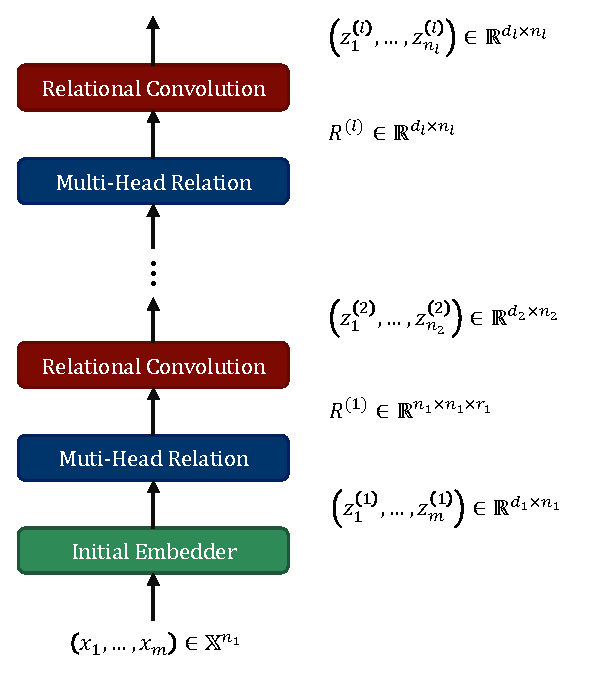
\includegraphics[width=.48\textwidth]{figs/relconv_architecture.pdf}
    \vskip-12pt
    \caption{Proposed architecture for relational convolutional networks. Hierarchical relations are modeled by iteratively computing pairwise relations between objects and convolving the resultant relation tensor with graphlet filters representing templates of relations between groups of objects.
    }\label{fig:relconv_architecture}
    % \vskip-12pt
\end{wrapfigure}

The key to the framework proposed in this paper involves formalizing the concept of convolving learnable templates of a relational pattern against a larger relation tensor. This operation produces a sequence of vectors representing the relational pattern within each group of objects. Crucially, composing relational convolutions captures higher-order relational features---i.e., relations between relations. Specifically, our proposed architecture introduces the following novel concepts and computational mechanisms.
\begin{itemize}%[itemsep=1pt]
    \item \textit{\bfseries Graphlet filters.} A ``graphlet filter'' is a template for the pattern of relations between a (small) collection of objects. 
    Since pairwise relations can be viewed as edges on a graph, the term ``graphlet'' is used to refer to a subgraph, and the term ``filter'' is used to refer to a learnable template or pattern.
    % Graphlet filters are analogous to filters (also called kernels) in traditional CNNs for images, which represent templates for local regions of an image.
    \item \textit{\bfseries Relational convolutions.} 
    We formalize a notion of \textit{relational} convolution, analogous to spatial convolutions in CNNs, where a graphlet filter is matched against the relations within \textit{groups} of objects to obtain a representation of the relational pattern in different groupings of the input.
    % In CNNs for image processing, each filter is
    %  ``swept,'' or 
    % spatially convolved across the image. For relational learning, we formalize an analogous notion of convolution where a graphlet filter can be matched against the relations between each group of objects.
    \item \textit{\bfseries Grouping mechanisms.} For large problem instances, it would be computationally and statistically intractable to consider relational convolutions across all combinations of objects. To achieve scalability, we introduce a learnable grouping mechanism based on attention which identifies the relevant groups that should be considered for the downstream task.
    \item \textit{\bfseries Compositional relational modules.} The proposed architecture supports composable modules, where each module has learnable graphlet filters and groups. This enables learning higher-order relationships between objects---relations between relations.
    % ---that are analogous to the composed feature maps that are of the essence in CNNs.
\end{itemize}


The architecture is presented in detail in Sections~\ref{sec:mdipr} and~\ref{sec:relconv}, and a schematic of the proposed architecture is shown in~\Cref{fig:relconv_architecture}. In a series of experiments, we show how relational convolutional networks provide a powerful framework
% and inductive bias 
for relational learning. We first carry out experiments on the ``relational games'' benchmark for relational reasoning proposed by~\citet{shanahanExplicitlyRelationalNeural}, which consists of a suite of binary classification tasks for identifying abstract relational rules between a set of geometric objects represented as images. 
We next carry out experiments on a version of the \textit{SET} game, which requires processing of higher-order relations across multiple attributes. We find that relational convolutional networks outperform transformers, graph neural networks, as well as existing relational architectures. We argue that these results demonstrate that both compositionality and relational inductive biases are needed to efficiently learn representations of complex higher-order relations.

\subsection{Related Work}\label{ssec:related_work}

To place our framework in the context of previous work, we briefly discuss related forms of relational learning below, pointing first to the review of relational learning inductive biases by~\cite{battagliaRelationalInductiveBiases2018}%,palmRecurrentRelationalNetworks2018,zhangRAVENDatasetRelational2019}. % battaglia is a review of "relational inductive biases" (though in a somewhat different sense to us). the rest are more specific, so this may not be the best place to cite them.

{Graph neural networks} (GNNs) are a class of neural network architectures which operate on graphs and process ``relational'' data~\citep[e.g.,][]{niepertLearningConvolutionalNeural2016,kipfSemiSupervisedClassificationGraph2017,schlichtkrullModelingRelationalData2017,velickovicGraphAttentionNetworks2017,kipfNeuralRelationalInference2018,xuHowPowerfulAre2018}. A defining feature of GNN models is their use of a form of neural message-passing, wherein the hidden representation of a node is updated as a function of the hidden representations of its neighbors on a graph~\cite{gilmerNeuralMessagePassing2017}. Typical examples of tasks which GNNs are applied to include node classification, graph classification, and link prediction~\cite{hamiltonGraphRepresentationLearning2020}. %This is a very general model which includes as a special case convolutional neural networks, where the graph is a grid, and Transformers, where the graph is a complete graph and the message-passing function is a convex sum of the neighbors' representations.

In GNNs, the `relations' are given to the model via edges in a graph. In contrast, our architecture, as well as the explicitly relational architectures described below, operate on collections of objects without any relations given as input. Instead, such relational architectures must infer the relevant relations from the objects themselves. Still, graph neural networks can be applied to these relational tasks by passing in the collection of objects along with a complete graph. % A Transformer Encoder can be thought of as a special case of this architecture.%, and hence is the representative baseline we compare against in our experiments.

Several works have proposed architectures with the ability to model relations by incorporating an {attention mechanism}~\citep[e.g.,][]{vaswani2017attention,velickovicGraphAttentionNetworks2017,santoroRelationalRecurrent2018,zambaldiDeepReinforcementLearning2018,locatelloObjectCentricLearningSlot2020}. Attention mechanisms, such as self-attention in Transformers~\citep{vaswani2017attention}, model relations between objects implicitly as an intermediate step in an information-retrieval operation
% a form of neural message-passing in order 
to update the representation of each object as a function of its context.

There also exists a growing literature on neural architectures which aim to explicitly model relational information between objects. An early example is the relation network proposed by~\citet{santoroSimpleNeural2017}.~\citet{shanahanExplicitlyRelationalNeural} proposes the PrediNet architecture, which aims to learn relational representations which are compatible with predicate logic.
% \todo{removed citation of ESBN for space (since not in baselines). can put back in camera-ready.}
% ~\citet{webbEmergentSymbols2021} proposes ESBN, a recurrent neural network augmented with external memory whose memory-write operation aims to factors representations into `sensory' and `relational'.
~\citet{kergNeuralArchitecture2022} proposes CoRelNet, a simple architecture based on `similarity scores' which aims to distill the relational inductive biases discovered in previous work into a minimal architecture.~\citet{altabaaAbstractorsTransformer2023} explored relational inductive biases in the context of Transformers, and proposed a view of relational inductive biases as a type of selective ``information bottleneck'' which disentangles relational information from object-level features.~\citet{webbRelationalBottleneckInductive2023} provides a cognitive science perspective on this idea, arguing that a relational information bottleneck may be a mechanism for abstraction in the human mind.% and brain.



\section{Multi-Head Relational Layer: modeling relations via inner products}\label{sec:mhr}

A relation function is a function which maps a pair of objects $o_1, o_2 \in \calX$ to a vector representing the relation between the two objects. For example, a relation may represent the information ``object 1 has the same color as object 2'', ``object 1 is larger than object 2'', and ``object 1 is to the left of object 2''. In principle, this can be modeled by an arbitrary learnable function on the concatenation of the two objects' representations. For example,~\citep{santoroSimpleNeural2017} models relations by MLPs applied to the concatenation of pairs of objects, $g_\theta(o_1, o_2)$. While this approach may work in some cases, it is missing some crucial inductive biases. In particular, there is no restriction that the learned pairwise function is in fact \textit{relational}. That is, $g_\theta(o_1, o_2)$ may just as well represent non-relational information like ``$o_1$ is bright'' and ``$o_2$ is small'', as opposed to relational information like ``$o_1$ is the same color as $o_2$'' and ``$o_1$ is larger than $o_2$''.

Recent work has explored using \textit{inner products} to model relations between objects~\citep{webbEmergentSymbols2021, kergNeuralArchitecture2022, altabaaAbstractorsTransformer2023}. The advantage of such an approach is that it provides added pressure to learn explicitly relational functions. In particular, it induces a geometry on the object space $\calX$ which allows objects to be described in relation to each other. To see this, we can first consider the case of symmetric relations modeled as inner products between feature maps. Let $\phi: \calX \to \reals^d$ be some feature map which represents a particular attribute of the object (e.g., color). Then, the inner product $\iprod{\phi(o_1)}{\phi(o_2)}$ induces a metric on $\calX$. In fact, $\iprod{\phi(o_1)}{\phi(o_2)}$ turns $\calX$ into an inner product space with well-defined notions of distance, angles, and orthogonality. Thus, we can say that the attribute $\phi$ is similar between two objects $o_1, o_2$ when the inner product $\iprod{\phi(o_1)}{\phi(o_2)}$ is large.

More generally, we can allow for multi-dimensional relations by having multiple encoding functions prior to the inner product. Furthermore, we can allow for asymmetric relations by having different encoding functions for the first and second object. This is the approach we take in~\citep{altabaaAbstractorsTransformer2023}. In particular, we model relations by,
\begin{equation}\label{eq:relation_function}
    r(x, y) = \begin{pmatrix}
        \iprod{\phi_1(x)}{\psi_1(y)} \\
        \vdots \\
        \iprod{\phi_{d_r}(x)}{\psi_{d_r}(y)}
    \end{pmatrix} \in \reals^{d_r},
\end{equation}

\noindent where $\phi_1, \psi_1, \ldots, \phi_{d_r}, \psi_{d_r}$ are learnable functions. For each dimension $k \in [d_r]$ of the relation function, the maps $\phi_k, \psi_k$ extract a particular attribute of the objects which is then compared by the inner product.

To promote weight sharing, we can have one common non-linear map $\phi$ across all dimensions along with different linear maps for each object and each dimension of the relation. That is,

\begin{equation}\label{eq:relation_function_lin_proj}
    r(x, y) = \begin{pmatrix}
        \iprod{W_1^{(1)}\phi(x)}{W_2^{(1)}\phi(y)} \\
        \vdots \\
        \iprod{W_1^{(d_r)}\phi(x)}{W_2^{(d_r)}\phi(y)} \\
    \end{pmatrix},
\end{equation}

\noindent where the learnable parameters are $\phi$ and $W_1^{(k)}, \ldots, W_1^{(k)}, k \in [d_r]$. $\phi: \calX \to \reals^{d_\phi}$ may be an MLP, for example, and $W_1^{(k)}, W_2^{(k)}$ are $d_i \times d_\phi$ matrices. The class of functions realizable by~\Cref{eq:relation_function_lin_proj} is the same as~\Cref{eq:relation_function} but enables greater weight sharing.

The ``Multi-Head Relation'' module receives a sequence of objects $x_1, \ldots, x_m$ as input and models the pairwise relations between them by~\Cref{eq:relation_function_lin_proj}, returning an $m \times m \times d_r$ relation tensor describing the pairwise relations between each pair of objects.

\subsection{Universal approximation of inner product relations}

\texttt{TODO: state result and cite writeup of these results.}

\section{Relational convolutions with graphlet filters}\label{sec:relconv}

\subsection{Relational convolutions with discrete groups}
Suppose that we have a sequence of objects $(x_1, \ldots, x_n)$ and a relation tensor $R$ describing the pairwise relations between them (obtained by a MD-IPR layer). The relational convolution operation we will define does two things: 1) extracts representations of the relational patterns within \textit{groups} of objects using pairwise relations, and 2) transforms the relation tensor back into a sequence of objects, allowing it be composed with another relational layer to compute higher-order relations.

Fix some filter size $s < n$, where $s$ is a hyperparameter of the relational convolution layer. One `filter' is given by the \textit{graphlet} $f_1 \in \mathbb{R}^{s \times s \times d_r}$. This is a `template' for the pairwise relations between $s$ objects. Note that the dimension of the relations in this filter matches that of the input relation tensor. Let $g \subset [n]$ be a subset of the objects of size $s$. Suppose for now that $g$ is an ordered set (i.e., the group $(1, 2, 3)$ is different from the group $(2, 3, 1)$). Then, denote the relation sub-tensor given by this (ordered) subset by $R[g] := [R[i,j]]_{i,j \in g}$. We define the `relational inner product' between this relation subtensor and the filter $f_1$ by
\begin{equation}
    \label{eq:relational_inner_prod_one_filt}
    \reliprod{R[g]}{f_1} \coloneqq \sum_{i,j \in g} \iprod{R[i,j]}{f_1[i,j]}_{\reals^{d_r}} = \sum_{i,j \in g} \sum_{k \in [d_r]} R[i,j,k] f_1[i,j,k].
\end{equation}
This is simply the inner product in the corresponding euclidean space $\mathbb{R}^{s^2 d_r}$. This quantity represents how much the relations within the objects in $g$ match the relations in the template $f_1$.

% Another relevant configuration is when the relation tensor $R$ is assumed to be symmetric (i.e.: pairwise relations are symmetric). In this case, filters can be restricted to be symmetric, and can now be identified with the smaller space $\{f \in \mathbb{R}^{s \times s \times r}: f[i,j] = f[j,i] \ \forall i,j \}$. The definition of the relational inner product can be simplified in this case to $\langle R[g], f_1 \rangle_R \coloneqq \sum_{i \leq j \in g} \langle R[i,j], f_1[i,j] \rangle$.

The relational convolution layer has $n_f$ filters (a hyperparameter). Denote the collection of filters by $\boldsymbol{f} = \paren{f_1, \ldots, f_{n_f}} \in \reals^{s \times s \times d_r \times n_f}$, which we call a \textit{graphlet filter}. We define the relational inner product of a relation subtensor $R[g]$ with a graphlet filter $\bm{f}$ as the $n_f$-dimensional vector consisting of the relational inner products with each individual filter,
\begin{equation}
    \label{eq:relational_inner_prod}
    \reliprod{R[g]}{\bm{f}} \coloneq \begin{pmatrix} \reliprod{R[g]}{f_1} \\ \vdots 
 \\ \reliprod{R[g]}{f_{n_f}} \end{pmatrix} \in \mathbb{R}^{n_f}.
\end{equation}
This vector summarizes various aspects of the relations within a group, captured by several different filters\footnote{We have overloaded notation, but will use the convention that a collection of filters is denoted by a bold symbol to distinguish between the two forms of the relational inner product.}.Each filter corresponds to one dimension in the final relation-summarizing vector for the group $g$. This is reminiscent of convolutional neural networks, where each filter gives us one channel in the output tensor.

We can also define a symmetric variant of the relational inner product which is invariant to the ordering of the elements in $g$. This can be done by pooling over all permutations of $g$. In particular, we suggest max-pooling and average-pooling, although any set-aggregator would be valid. We denote the permutation-invariant relational inner product by $\iprod{R[g]}{f_1}_{\mathrm{rel}, \mathrm{sym}}$,
\begin{equation}\label{eq:symmetric_relational_inner_prod}
    \iprod{R[g]}{\bm{f}}_{\mathrm{rel}, \mathrm{sym}} \coloneq \mathrm{Pool}\paren{\set{\reliprod{R[g']}{\bm{f}} \colon g' \in g!}},
\end{equation}
\noindent where $g!$ denotes the set of permutations of the group $g$. Recall that each $\iprod{R[g']}{\bm{f}}_{\mathrm{rel}}$ is $n_f$-dimensional, and the pooling is done independently for each dimension.

For a given group $g \subset [n]$, the relational inner product with a graphlet filter, $\iprod{R[g]}{\bm{f}}_\mathrm{rel}$, gives us a vector summarizing the relational patterns inside that group. We aim to get a sequence of objects which each describes the relational patterns within each group of interest. Let $\calG$ be a set of size-$s$ groups of the the $n$ objects. The relational convolution between a relation tensor $R$ and a relational graphlet filter $\bm{f}$ is the sequence of relational inner products with each group in $\calG$,
\begin{equation}
    \label{eq:relational_convolution}
    R \ast \bm{f} \coloneq \left( \reliprod{R[g]}{\boldsymbol{f}} \right)_{g \in \calG} \equiv \left(z_1, \ldots, z_{\abs{\calG}}\right) \in (\mathbb{R}^{n_f})^{\abs{\calG}}
\end{equation}
$\calG$ is a pre-specified hyperparameter of the relational convolution operation. The choice depends on the usecase. If some prior information is known about reasonable groupings, this can be encoded in $\calG$. When $n$ is small and no prior information is available, a reasonable choice might be the the set of all combinations of size $s$. When $n$ is large, considering all combinations will be intractable. One solution is to consider a random sample of combinations. In the next subsections, we consider the problem of \textit{learning} the relevant groups.

% In the above, we either consider all possible groups or we somehow assume that the relevant groups $\calG$ are known and given. We may also wish to \textit{learn} the relevant groups.

\begin{figure}
    \vskip-10pt
    \centering
    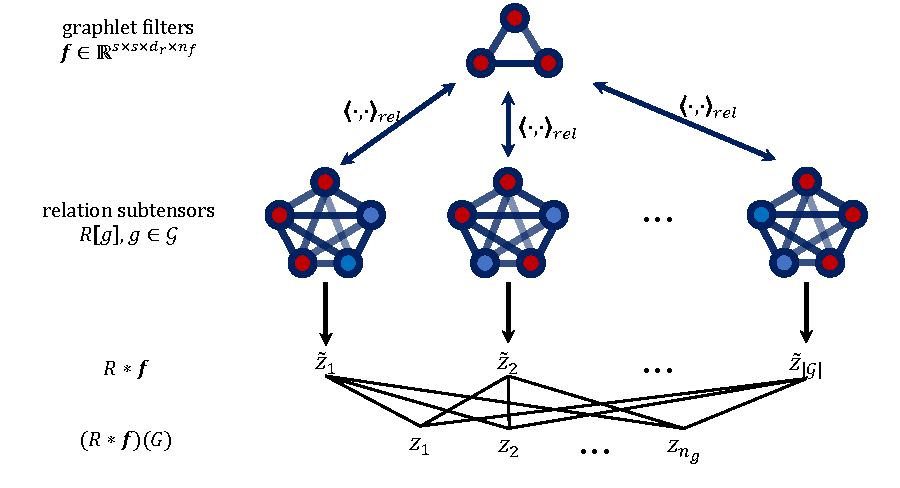
\includegraphics[width=0.9\textwidth]{figs/relconv_diagram2.pdf}
    \vskip-10pt
    \caption{A depiction of the relational convolution operation.
    % NOTE / TODO temporarily add? (reviewer asked for this but we're tight on space)
    % The input is a relation tensor $R \in \reals^{n \times n \times d_r}$. A learned set of graphlet filters $\bm{f} \in \reals^{s \times s \times d_r \times n_f}$ are compared to each relation subtensor $R[g], g \in \calG$, producing the relational convolution $R \ast \bm{f}$. With a group matrix $G \in \reals^{m \times n_g}$, $(R \ast \bm{f})(G)$ represents the relational information in a set of $n_g$ ``soft groups''.
    % The input is a relation tensor $R$ of shape $m \times m \times d_r$, giving pairwise relations of dimension $d_r$ between a sequence of $m$ objects. A graphlet filter of size $s$ is parameterized by a relation tensor of shape $s \times s \times d_r$. The graphlet convolution operation computes relational inner products between the relation subtensor of each discrete group $g \in \calG$ with the graphlet filters $\bm{f}$. This gives a vector representation of the relations in each discrete group, $\tilde{z}_g \in \reals^{n_f}, g \in \calG$. Finally, this is synthesized into a vector representation for each of $n_g$ `soft groups', $G$, producing $(R \ast \bm{f})(G) = (z_1, \ldots, z_{n_g})$.
    }\label{fig:relconvdiagram}
    \vskip -10pt
\end{figure}

\subsection{Relational convolutions with `soft' groups}

In the above formulation, the groups are `discrete'. Having discrete groups can be desirable for interpretability, if the relevant groupings are known a priori or if considering every possible grouping is computationally and statistically feasible. However, if the relevant groupings are not known, then considering all possible combinations results in a rapid growth of the number of objects at each layer.
% Besides being computationally intractable, considering every possible grouping may be unnecessary and may make learning more difficult.

In order to address these issues, we propose \textit{explicitly modeling groups}. This allows us to control the number of objects in the output sequence of a relational convolution operation such that only relevant groups are considered. In the next section, we outline some ways to model `soft groups' using \textit{grouping layers}. These layers take a sequence of objects and/or the relation tensor as input and produce a `group matrix' $G \in \reals^{n \times n_g}$ representing $n_g$ `soft groups'. The $(i,j)$-th entry of the group matrix represents the degree to which the $i$-th object belongs to the $j$-th group. The number of groups $n_g$ is a configurable hyperparameter of the grouping layers. For the remainder of this subsection, we assume that the group matrix $G$ is given as input to the relational convolution layer.

Consider the group matrix $G \in \reals^{n \times n_g}$ and filters $\bm{f}$ of size $s$. First, we use $G$ to compute a ``group-match score'' for each discrete group $g$ of size $s$ (e.g., $g \in \calG = \binom{[n]}{s}$). This is done via
\begin{equation}\label{eq:group_match_score}
    \begin{split}
        G &\gets \text{SoftPlus}(G)\\
        \alpha_{gk} &\gets \text{Normalize}\paren{\bra{\prod_{i \in g} G[i,k]}_{g \in \calG}}, \quad g \in \calG, k \in [n_g],
    \end{split}
\end{equation}
where the soft-plus function is $\text{Softplus}(x) = \log(\exp(x + 1))$, applied elementwise. This has the effect of making the group matrix $G$ non-negative which is needed for the product of its elements to represent a ``group-match score''. The product inside the softmax is over elements in the discrete group $g \in \calG$. Hence, it will be large whenever the soft group $G_k := G[:, k]$ aligns with the discrete group $g$. $\mathrm{Normalize}(\cdot)$ normalizes the group match scores so that $\sum_{g} \alpha_{gk} = 1$. We propose the use of sparse normalizers~\citep{lahaControllableSparseAlternatives2018a} so that only a sparse subset of discrete groups in $\calG$ contribute to each soft group (see also~\Cref{ssec:computational_considerations}). In our experiments, we use `sparsemax'~\citep{martinsSoftmaxSparsemaxSparse2016}. Thus, $\alpha_{gk}$ is a normalized ``group-match score'' indicating the degree to which the discrete group $g$ matches the given soft group $G_k$.
% \footnote{Sparse normalizers would likely be appropriate alternatives to softmax here, since it would be desirable to have only a sparse subset of discrete groups in $\calG$ contribute to each soft group. Some sparse alternatives to softmax are discussed in~\citep{lahaControllableSparseAlternatives2018a}.}. %Note that the group match scores of discrete groups sum to one, $\sum_{g \in G} \alpha_{gk} = 1, \ \forall k \in [n_g]$.

Now, we can define the `soft' relational inner product \textit{given} the soft group $G_k$ by
\begin{equation}\label{eq:soft_relational_inner_prod}
    \langle R, \boldsymbol{f} \, \vert \, G_k \rangle_R \coloneqq \sum_{g \in \calG} \alpha_{gk} \iprod{R[g]}{\boldsymbol{f}}_\mathrm{rel}.
\end{equation}
This notation should be read as ``the relational inner product of the relation tensor $R$ with the graphlet filters $\boldsymbol{f}$ given the group $G_k$''. This expression is essentially a convex combination of the relational inner product with all possible discrete groups weighted by how much they match the soft group $G_k$.

With this modification, the number of objects in the output sequence is fixed and controlled by the number of groups, $n_g$ (which is a hyperparameter). The output sequence of the relational convolution given groups $G$ is now given by
\begin{equation}\label{eq:soft_relational_convolution_groups}
    (R \ast \bm{f})(G) = \left( \softreliprod{R}{\bm{f}}{G_1}, \ldots, \softreliprod{R}{\bm{f}}{G_{n_g}} \right) \in \left(\mathbb{R}^{n_f}\right)^{n_g}.
\end{equation}

\subsection{Relational convolutions with group attention \textcolor{red}{[ALTERNATIVE]}}

In the above formulation, the groups are `discrete'. Having discrete groups can be desirable for interpretability, if the relevant groupings are known a priori or if considering every possible grouping is computationally and statistically feasible. However, if the relevant groupings are not known, then considering all possible combinations results in a rapid growth of the number of objects at each layer.
% Besides being computationally intractable, considering every possible grouping may be unnecessary and may make learning more difficult.

In order to address these issues, we propose \textit{explicitly modeling groups}. This allows us to control the number of objects in the output sequence of a relational convolution operation such that only relevant groups are considered. We propose modeling groups via an \textit{attention} operation.

Consider the input $X = \paren{x_1, \ldots, x_n},\, x_i \in \reals^d$. Let $n_g$ be the number of groups to be learned and $s$ be the size of the graphlet filter, which are hyperparameters to the model. We learn $n_g \times s$ group query vectors $Q = \{q_{i}^{g}\}_{g \in [n_g], i \in [s]}$. That is, for each group $g \in [n_g]$, we learn $s$ queries which will be used to retrieve a group of size $s$ via attention. The $i$-th object in the $k$-th group is retrieved via an attention operation as follows,
\begin{equation}\label{eq:group_attn}
    \begin{aligned}
        \bar{x}_{i}^{g} &= \sum_{j = 1}^{n} \alpha_{ij}^{g} x_j, \ &&g \in [n_g],  i \in [s]\\
        \alpha_{ij}^{g} &= \frac{\exp\paren{\beta \iprod{q_i^g}{\mathtt{key}(x_j)}}}{\sum_{k = 1}^{n}{\exp\paren{\beta \iprod{q_i^g}{\mathtt{key}(x_k)}}}}, \ &&k \in [n_g], i \in [s], j \in [n]
    \end{aligned}
\end{equation}
where $\bar{x}_{i}^{g}$ is the $i$-th object in the $g$-th group, $q_{i}^{g}$ is the query for retrieving the $i$-th object in the $g$-th group, $\mathtt{key}(x_j)$ is the key associated with the object $x_j$, and $\beta$ is a learnable scaling parameter.

The $\mathtt{key}$ for each object is computed as a function of its position, features, and/or context. For example, to group objects based on their position, the key can be a positional embedding. To group based on features, the $\mathtt{key}$ can be a linear projection of the object's feature vector. To group based on both position and features, the $\mathtt{key}$ can be a sum or concatenation of the above. Finally, groups can also be modeled based on contextual information by computing keys through a self-attention operation.

\Cref{eq:group_attn} can be computed in parallel with an `einsum' operation in $\calO(n \cdot n_g \cdot s \cdot d)$ operations. When the hyperparameters of the model are fixed, this is linear in the sequence length $n$.

The relation subtensor $\bar{R}[g] \in \reals^{s \times s \times d_r}$ for each group $g \in [n_g]$ is then computed using a shared MD-IPR layer $r(x, y)$,
\begin{equation}
    \bar{R}[g]_{ij} = r(\bar{x}_{i}^{g}, \bar{x}_{j}^{g}).
\end{equation}
This computation can be carried out in parallel via efficient matrix multiplication with $\calO(n_g \cdot s^2 \cdot d_r \cdot d_{\mathrm{proj}})$ operations. Note that This does not scale with the number of objects in the input, and is only a function of the hyperparameters of the model. Moreover, the filter size $s$ is typically of very modest size (e.g., $3$ or $5$).

The relational convolution is computed as before via,
\begin{equation}
    \bar{R} \ast \bm{f} \equiv \paren{\reliprod{\bar{R}[g]}{\bm{f}}}_{g \in [n_g]}.
\end{equation}

Overall, relational convolution with group attention can be summarized as follows: 1) learn $n_g$ groupings of objects, retrieving $s$ objects per group; 2) compute the relation tensor of each group using a MD-IPR module; 3) compute a relational convolution with a learned set of graphlet filters $\bm{f}$, producing a sequence of $n_g$ vectors each describing the relational pattern within a (learned) group of objects.

The group attention scores in~\Cref{eq:group_attn} are ideally close to discrete assignments. That is, the vector $\alpha_{i,\cdot}^{g} \in \Delta^{n}$ is ideally a one-hot vector for each $g \in [n_g],\, i \in [s]$. To encourage the model to learn more structured group assignments, we add an entropy regularization to the loss function, $\calL_{\mathtt{entr}} = \frac{1}{n_g \cdot s} \sum_{g, i} H(\alpha_{i,\cdot}^{g})$, where $H(\alpha_{i,\cdot}^{g}) = - \sum_{j} \alpha_{ij}^{g} \log(\alpha_{ij}^g)$ is the Shannon entropy. As a heuristic, this regularization can be scaled by $\sim \log(\mathtt{n\_classes}) / \log(n)$ so that it doesn't dominate the underlying task's loss.

\section{Grouping Layers}\label{sec:grouping_layers}

A grouping layer is a layer which outputs a group matrix $G \in \reals^{m \times n_g}$ representing the degree to which each object $i \in [m]$ belongs to each group $j \in [n_g]$. The number of groups $n_g$ is a configurable hyperparameter. We briefly describe some proposals for grouping layers with different properties.

\textbf{Temporal Grouping.} In the temporal grouping layer, the groups are a function only of the temporal order of the objects. This can be achieved by learning the group matrix $G$ directly as a parameter of the model. $G$ will be optimized along with the rest of the model parameters as a function of its effect on the relational convolution layer. Temporal grouping would be appropriate in situations where the order in which objects appear is predetermined and indicates the relevant groups.

\textbf{Feature-based Grouping.} In a feature-based grouping layer, the group(s) to which each object belongs is a function of that object's features (and position). That is,
\begin{equation}
        G \gets \begin{bmatrix}
            \phi(1, x_1)^\top \\
            \vdots \\
            \phi(m, x_m)^\top
        \end{bmatrix} \in \reals^{m \times n_g},
\end{equation}

\noindent where $\phi: [m] \times \calX \to \reals^{n_g}$ is a learnable function which maps an object's temporal order $i$ and feature representation $x_i$ to a $n_g$-dimensional group membership vector where the $j$th entry of the vector represents the degree to which the object belongs to the $j$th group. For example $\phi$ can be a multi-layer perceptron of the form $\phi(i, x) = \mathrm{MLP}(\mathrm{concat}(e_i, x))$. Feature-based grouping may be useful in situations where group membership can be determined for each object using only that object's features, irrespective of the context of the other objects in the sequence.

\textbf{Context-aware Grouping.} In some applications, the group(s) to which each object belongs to may depend on the full context of the other objects in the sequence. One way to model this is to use a message-passing neural network to update the representations of each object, incorporating the context of the other objects in the sequence. Then, a multi-layer perceptron is applied to each encoded object to produce the group membership vector for that object.
\begin{equation}
    \begin{split}
        E_i &\gets \mathrm{MessagePassing}\paren{x_i, \set{x_1, \ldots, x_m}}, \ i \in [m] \\
        G &\gets \begin{bmatrix}\mathrm{MLP}(E_1)^\top \\ \vdots \\ \mathrm{MLP}(E_m)^\top \end{bmatrix} \in \reals^{m \times n_g}.
    \end{split}
\end{equation}

This is the most general form of grouping, as it encompasses the previous two forms as special cases. The updated representation of each object $E_i$ now contains any relevant information about the other objects which should be considered in computing its group membership vector. One simple and effective option for the message-passing operation is to use self-attention. In this case, since a multi-head relational layer precedes the relational convolution layer, the relation tensor can be re-used in the self-attention operation to compute attention scores.

\section{Experiments}\label{sec:experiments}

\texttt{[TODO]}

\texttt{Description of relational games}

\begin{table}
    \centering
    \begin{tabular}{llll}
\toprule
              &             &     Hexos Accuracy &   Stripes Accuracy \\
Task & Model &                    &                    \\
\midrule
same & RelConvNet &  $0.989 \pm 0.002$ &  $0.974 \pm 0.003$ \\
              & CoRelNet &  $0.988 \pm 0.006$ &  $0.724 \pm 0.112$ \\
              & PrediNet &  $0.990 \pm 0.004$ &  $0.983 \pm 0.007$ \\
              & Transformer &  $0.997 \pm 0.001$ &  $0.993 \pm 0.004$ \\\hline
occurs & RelConvNet &  $0.980 \pm 0.001$ &  $0.880 \pm 0.015$ \\
              & CoRelNet &  $0.992 \pm 0.004$ &  $0.518 \pm 0.012$ \\
              & PrediNet &  $0.907 \pm 0.020$ &  $0.775 \pm 0.046$ \\
              & Transformer &  $0.881 \pm 0.015$ &  $0.724 \pm 0.021$ \\\hline
xoccurs & RelConvNet &  $0.967 \pm 0.001$ &  $0.946 \pm 0.006$ \\
              & CoRelNet &  $0.980 \pm 0.007$ &  $0.606 \pm 0.035$ \\
              & PrediNet &  $0.872 \pm 0.036$ &  $0.810 \pm 0.028$ \\
              & Transformer &  $0.867 \pm 0.017$ &  $0.753 \pm 0.031$ \\\hline
between & RelConvNet &  $0.991 \pm 0.001$ &  $0.988 \pm 0.002$ \\
              & CoRelNet &  $0.995 \pm 0.001$ &  $0.582 \pm 0.063$ \\
              & PrediNet &  $0.978 \pm 0.006$ &  $0.950 \pm 0.019$ \\
              & Transformer &  $0.986 \pm 0.003$ &  $0.961 \pm 0.010$ \\\hline
match pattern & RelConvNet &  $0.961 \pm 0.015$ &  $0.870 \pm 0.041$ \\
              & CoRelNet &  $0.942 \pm 0.011$ &  $0.581 \pm 0.026$ \\
              & PrediNet &  $0.710 \pm 0.040$ &  $0.658 \pm 0.053$ \\
              & Transformer &  $0.627 \pm 0.005$ &  $0.591 \pm 0.006$ \\
\bottomrule
\end{tabular}

    \caption{Out-of-distribution Generalization results on relational games.}
\end{table}

% \section{Function Class of Multi-Head Relation Module}\label{mhr_function_class}

In previous work, we characterized the class of functions which can be modeled by \textit{symmetric} multi-head relation modules~\citep{altabaaAbstractorsTransformer2023}. In particular, we showed that this class of functions is the set of relation functions which are symmetric kernels of positive type (i.e., Mercer kernels) in each relation dimension.

Symmetric relation functions modeled in this way are natural \textit{measures of similarity}. To see this, suppose we have a normalized symmetric positive definite kernel $K$, such that $K(x,x) = 1$ for all $x \in \calX$. Then, the Cauchy-Schwarz inequality for Mercer kernels states that
\begin{equation}
    K(x, y)^2 \leq K(x, x) K(y, y) = 1, \ \forall x, y \in \calX.
\end{equation}

Thus, $K(x,y)$ is large and close to $1$ when $x$ and $y$ are similar, and close to $0$ when $x, y$ are dissimilar. 

In some applications (e.g., where the relations are indeed measures of `similarity'), this property will be desirable and hence modeling relations as symmetric will be a useful inductive bias. However, in other applications, this may be a restrictive assumption---the underlying relations may be more complex than simple measures of similarity. In such cases, we don't want to restrict the modeled relations to be symmetric and positive definite. In this section, we characterize the class of functions which can be modeled by multi-head relation modules and prove a universal approximation result stating that this includes any continuous function on $\calX \times \calX$. We begin by drawing a connection to reproducing kernel Banach spaces. This is a generalization of reproducing kernel Hilbert spaces which is what we used in our earlier analysis in~\citep{altabaaAbstractorsTransformer2023}.


\subsection{Background on reproducing kernel Banach spaces}

Recall that a reproducing kernel hilbert space (RKHS) $\calH$ is a hilbert space of functions on a space $\calX$ in which the point evaluation functionals $f \mapsto f(x)$ are continuous. There is a one-to-one identification between RKHSs and symmetric positive definite kernels $K: \calX \times \calX \to \reals$ such that $\iprod{K(x, \cdot)}{f}_\calH = f(x)$ \citep{moore-aronszajn}. \citep{mercerFunctionsPositive1909} further shows that an RKHS can be identified with a feature map via the spectral decomposition of the integral operator $T_K: L_2(\calX) \to L_2(\calX)$ defined by $T_K f(x) = \int_\calX K(x, y) f(y) dy$. Every feature map $\phi: \calX \to \calW$ defines a symmetric positive definite kernel $K(x, y) = \iprod{\phi(x)}{\phi(y)}_\calW$ (hence, an RKHS) and every symmetric positive definite kernel has infinitely many feature map representations.

As discussed above, modeling relations as symmetric positive definite kernels may be restrictive in some applications. Hence, we choose to model relations as multi-dimensional asymmetric functions, while maintaining the inductive bias of modeling relations as inner products.
\begin{equation*}
    r(x,y) = \begin{pmatrix} \iprod{\phi_1(x)}{\psi_1(y)} \\ \vdots \\ \iprod{\phi_{d_r}(x)}{\psi_{d_r}(y)}\end{pmatrix}
\end{equation*}

To analyze the class of functions realizable by such models, we make use of another tool in functional analysis: reproducing kernel \textit{Banach} spaces (RKBS) \citep{zhangReproducingKernel2009}. RKBS generalize RKHS, allowing for a richer class of kernels. We begin by presenting some of the relevant background on RKBS before proceeding to analyze the function class of multi-head relation modules.

\begin{definition}[Reproducing Kernel Banach Space]
    A \textbf{reproducing kernel Banach space} on a space $\calX$ is a Banach space $\calB$ of functions on $\calX$, satisfying:
    \begin{enumerate}
        \item $\calB$ is \textit{reflexive}. That is, $(\calB^*)^* = \calB$, where $\calB^*$ is the dual space of $\calB$. Furthermore, $\calB^*$ is isometric to a Banach space $\calB^\#$ of functions on $\calX$.
        \item The point evaluation functionals $f \mapsto f(x)$ are continuous on both $\calB$ and $\calB^\#$.
    \end{enumerate}
\end{definition}

This definition is a strict generalization of reproducing kernel Hilbert spaces, as any RKHS $\calH$ on $\calX$ is also an RKBS ((1) is satisfied by the Riez representation theorem). While the identification $\calB^\#$ is not unique, we can choose some identification arbitrarily and denote it by $\calB^*$ for ease of notation (by assumption, all identifications are isometric to each other). Thus, if $\calB$ is an RKBS, $\calB^*$ is also an RKBS.

Similar to an RKHS, an RKBS also has a \textit{reproducing kernel}. To state the result, for a normed vector space $\calV$ and its dual space $\calV^*$, we define the bilinear form
\begin{equation}\label{eq:bilinear_form}
    \begin{split}
        \calV \times \calV^* &\to \reals\\
        (u, v^*)_\calV &\mapsto v^*(u).
    \end{split}
\end{equation}

\citep[Theorem 2]{zhangReproducingKernel2009} shows that for any RKBS $\calB$ there exists a unique reproducing kernel $K: \calX \times \calX \to \bbC$ which recovers point evaluations,
\begin{align}
    f(x) &= \paren{f, K(\cdot, x)}_\calB, \forall f \in \calB, \\
    f^*(x) &= \paren{K(x, \cdot), f^*}_\calB \forall f^* \in \calB^*,
\end{align}

and such that the span of $K(x, \cdot)$ is dense in $\calB$ and the span of $K(\cdot, x)$ is dense in $\calB^*$,
\begin{align}
    \overline{\text{span}}\{K(x, \cdot): x \in \calX\} &= \calB, \\
    \overline{\text{span}}\{K(\cdot, x): x \in \calX\} &= \calB^*.
\end{align}

Finally,

\begin{equation}
    K(x, y) = \paren{K(x, \cdot), K(\cdot, y)}_\calB, \ \forall x, y \in \calX.
\end{equation}

Unlike RKHSs, while each RKBS has a unique reproducing kernel, different RKBSs may have the same reproducing kernels.

Furthermore,~\citep[Theorems 3 and 4]{zhangReproducingKernel2009} show that a kernel $K: \calX \times \calX \to \bbC$ is the reproducing kernel of some RKBS if and only if it has a feature map representation. Crucially for us, the feature map representation is more versatile than the one for RKHSs. Let $\calW$ be a reflexive Banach space with dual space $\calW^*$. Consider a pair of feature maps $\Phi$ and $\Phi^*$, mapping to each feature space, respectively. That is,
\begin{equation*}
    \Phi: \calX \to \calW, \ \Phi^*: \calX \to \calW^*,
\end{equation*}

\noindent where we call $\Phi, \Phi^*$ the \textit{pair} of feature maps and $\calW, \calW^*$ the pair of feature spaces. Suppose that the span of the image of the feature maps under $\calX$ is dense in their respective feature spaces. That is,
\begin{equation}
    \overline{\text{span}}\{\Phi(x): x \in \calX\} = \calW, \ \overline{\text{span}}\{\Phi^*(x): x \in \calX\} = \calW^*.
\end{equation}

Then, by~\citep[Theorem 3]{zhangReproducingKernel2009}, the feature maps $\Phi, \Phi^*$ induce an RKBS defined by

\begin{align}
    \calB &:= \set{f_w: x \mapsto (\Phi^*(x))(w), w \in \calW} \\
    \norm{f_w}_\calB &:= \norm{w}_\calW,
\end{align}

\noindent with the dual space $\calB^*$ defined by
\begin{align}
    \calB^* &:= \set{f_{w^*}: x \mapsto w^*(\Phi(x)), w^* \in \calW^*} \\
    \norm{f_{w^*}}_{\calB^*} &:= \norm{w^*}_{\calW^*}.
\end{align}

Furthermore, for any RKBS, there exists some feature spaces $\calW, \calW^*$ and feature maps $\Phi, \Phi^*$ such that the above construction yields that RKBS~\citep[Theorem 4]{zhangReproducingKernel2009}.

\subsection{MHR layers model kernels of reproducing kernel Banach spaces}

Observe that for a RKBS with feature-map representation given by $\Phi, \Phi^*$, it's reproducing kernel is given by
\begin{equation}
    K(x, y) = \paren{\Phi(x), \Phi^*(y)}_{\calW}, \ x, y \in \calX,
\end{equation}

\noindent where $\paren{\cdot, \cdot}_{\calW}$ is the bilinear form on $\calW$ defined in~\Cref{eq:bilinear_form}.

We motivate the following analysis by noting the similarity with our model of relation functions. Recall that the $k$-th dimension of the relation function $r: \calX \times \calX \to \reals^{d_r}$ is modeled as
\begin{equation}
    r_k(x, y) = \iprod{\phi_k(x)}{\psi_k(y)}, \ x, y \in \calX,
\end{equation}
\noindent where $\phi_k, \psi_k \to \reals^{d_r^{(k)}}$ is a pair of learned feature maps. Typically, $\phi_k, \psi_k$ are neural networks with vector outputs into the common feature space $\reals^{d_r^{(k)}}$.

\begin{theorem}\label{thm:mhr_approximates_rkbs}
   Suppose $\calX$ is a compact metric space. Suppose the ground truth relation function $r: \calX \times \calX \to \reals^{d_r}$ is such that each component $r_i$ is the reproducing kernel of some RKBS $\calB$ on $\calX$ which admits a feature map representation with a feature space $\calW$ which is a Hilbert space. Consider the model,

   \begin{equation}
    \tilde{r}(x, y) = \paren{\iprod{\phi_1(x)}{\psi_1(y)}, \ldots, \iprod{\phi_{d_r}(x)}{\psi_{d_r}(y)}},
   \end{equation}

   \noindent where $\phi_i, \psi_i: \calX \to \reals^{d_r^{(i)}}$ are multi-layer perceptrons. Then, for any $\varepsilon > 0$, there exists multi-layer perceptrons with parameters $\theta_\phi^{(i)}, \theta_{\psi}^{(i)}, i \in [d_r]$ such that
   \begin{equation*}
        \sup_{x,y} \infnorm{r(x, y) - \tilde{r}(x, y)} \leq \varepsilon
   \end{equation*}
\end{theorem}

\begin{proof}
    \hphantom{~}

    We will focus on each dimension of the relation function's $d_r$ components individually. That is, we will show the existence of $\phi_i, \psi_i$ such that $\tilde{r}_i(x, y) = \iprod{\phi_i(x)}{\psi_i(y)}$ approximates $r_i$. By assumption, there exists a Hilbert space $\calW$ and a pair of feature maps $\Phi_i: \calX \to \calW, \Phi_i^*: \calX \to \calW$ such that,
    \begin{equation*}
        r_i(x, y) = \paren{\Phi(x), \Phi^*(y)}_{\calW} \equiv (\Phi^*(y))(x), \ x, y \in \calX.
    \end{equation*}

    By~\citep{}, any two Hilbert spaces with equal dimension are isometrically isomorphic. Hence, without loss of generality, we can restrict our attention to the feature space $\calW = \ell^2(\bbN)$. The dual space is $\calW^* = \ell^2(\bbN)$. Hence, for feature maps $\Phi_i, \Phi_i^*$, the ground truth relation to be approximated is,
    \begin{equation*}
        r_i(x, y) = \paren{\Phi_i(x), \Phi_i^*(y)}_{\ell^2(\bbN)} \equiv (\Phi_i^*(y))(\Phi_i(x)), \ x, y \in \calX.
    \end{equation*}

    By the Riesz representation theorem~\citep{riesz_citation}, there exists a unique element in $u_{\Phi^*(y)} \in \ell^2(\bbN)$ such that,
    \begin{equation*}
        (\Phi^*(y))(w) = \iprod{w}{u_{\Phi^*(y)}}_{\ell^2(\bbN)}, \ \forall w \in \ell^2(\bbN).
    \end{equation*}

    Let $\sigma: \ell^2(\bbN)^* \to \ell^2(\bbN)$ denote the mapping from an element in the dual space to its Riesz representation. $\sigma$ is a bijective isometric antilinear isomorphism. (e.g., the riesz representation can be cosntructed via an orthonormal basis through $\sigma(w^*) = \sum_{i \in I} w^{*}(e_i) e_i$, where $\set{e_i}_{i \in I}$ is some basis for $\calW$).

    Thus, the relation function on $\calX \times \calX$ that we need to approximate is,
    \begin{equation*}
        r_i(x, y) = \iprod{\sigma \circ \Phi_i^* (y)}{\Phi_i(x)}_{\calW}, \ x, y \in \calX.
    \end{equation*}

    We do this by approximating $\Phi_i: \calX \to \calW$ with the MLP $\psi_i$ and approximating $\sigma \circ \Phi_i^*: \calX \to \calW$ with the MLP $\phi_i$.

    First, since $\Phi_i(x), \sigma \circ \Phi^*_i(y) \in \ell^2(\bbN), \forall x, y$, and $\calX$ is compact, we have
    \begin{equation*}
        \lim_{n \to \infty} \sup_{x,y \in \calX} \abs{r_i(x, y) - \sum_{j=1}^{n} (\Phi_i(x))_j \cdot (\sigma(\Phi^*(y)))_j} = 0.
    \end{equation*}

    Thus, let $\tilde{n}_i$ be such that,
    \begin{equation}\label{eq:thm1_proof_eq1}
        \sup_{x,y \in \calX} \abs{r_i(x, y) - \sum_{j=1}^{\tilde{n}_i} (\Phi_i(x))_j \cdot (\sigma(\Phi^*(y)))_j} < \frac{\varepsilon}{2}.
    \end{equation}

    Now, let the $i$th MLPs, $\phi_i, \psi_i$ be functions from $\calX$ to $\reals^{\tilde{n}_i}$ (i.e., we specify the architecture of the MLPs such that the output space is $\tilde{n}_i$-dimensional). Let $\paren{(\Phi_i(x))_1, \ldots, (\Phi_i(x))_{\tilde{n}_i}}$ be the function to be approximated by the MLP $\phi_i$ and let $\paren{(\sigma(\Phi^*(y)))_1, \ldots, (\sigma(\Phi^*(y)))_{\tilde{n}_i}}$ be the function to be approximated by the MLP $\psi_i$. By universal approximation results on MLPs (e.g.,~\citep{barronUniversalApproximation1993, cybenkoApproximationSuperpositions1989, hornikMultilayerFeedforward1989}), for any $\tilde{\varepsilon} > 0$, there exists parameters $\theta_{\phi}^{(i)}, \theta_{\psi}^{(i)}$ such that,

    \begin{equation}\label{eq:thm1_proof_eq2}
        \sup_{x \in \calX} \abs{(\phi_i(x))_j - (\Phi_i(x))_{j}} < \tilde{\varepsilon} \ \text{ and } \ \sup_{x \in \calX} \abs{(\psi_i(y))_j - (\sigma(\Phi^*(x)))_{j}} < \tilde{\varepsilon}, \ \forall j \in \set{1, \ldots, \tilde{n}_i}.
    \end{equation}

    Now, 
    \begin{align*}
        &\sup_{x,y \in \calX} \abs{r_i(x,y) - \tilde{r}_i(x,y)} \\
        &= \sup_{x,y \in \calX} \abs{r_i(x,y) - \iprod{\phi_i(x)}{\psi_i(y)}} \\
        &\leq \sup_{x,y\in \calX} \paren{\abs{r_i(x,y) - \sum_{j=1}^{\tilde{n}_i} (\Phi_i(x))_j \cdot (\sigma(\Phi^*(y)))_j} + \abs{\sum_{j=1}^{\tilde{n}_i} (\Phi_i(x))_j \cdot (\sigma(\Phi^*(y)))_j - \iprod{\phi_i(x)}{\psi_i(y)}}} \\
    \end{align*}

    The first term is less than $\varepsilon / 2$ by~\Cref{eq:thm1_proof_eq1}. Now, we bound the second term uniformly on $x,y \in \calX$,
    \begin{align*}
        &\abs{\sum_{j=1}^{\tilde{n}_i} (\Phi_i(x))_j \cdot (\sigma(\Phi^*(y)))_j - \iprod{\phi_i(x)}{\psi_i(y)}} \\
        &\leq \sum_{j=1}^{\tilde{n}_i} \abs{(\Phi_i(x))_j \cdot (\sigma(\Phi^*(y)))_j - (\phi_i(x))_j(\psi_j(y))_j} \\
        &\leq \sum_{j=1}^{\tilde{n}_i} \abs{(\phi_i(x))_j} \abs{(\sigma(\Phi^*(y)))_j - (\psi_j(y))_j} + \abs{(\psi_i(y))_j} \abs{(\Phi_i(x))_j - (\phi_i(x))_j}\\
    \end{align*}

    Let $\tilde{\varepsilon}$ in~\Cref{eq:thm1_proof_eq2} be small enough such that the above is smaller than $\varepsilon / 2$. This shows that

    \begin{equation*}
        \sup_{x,y \in \calX} \abs{r_i(x,y) - \tilde{r}_i(x,y)} \leq \frac{\varepsilon}{2} + \frac{\varepsilon}{2} = \varepsilon.
    \end{equation*}

    We repeat this procedure to obtain the MLP parameters $\theta_\phi^{(i)}, \theta_{\psi}^{(i)}$ for each dimension $i = 1, \ldots, d_r$. Thus, the error is bounded for each dimension, and $\sup_{x,y} \norm{r(x, y) - \tilde{r}(x, y)}_2 \leq \varepsilon$.
\end{proof}

\begin{remark}
    The reason we assume that the underlying RKBS $\calB$ admits a feature map representation with feature space $\calW$ which is a Hilbert space is so that we can use the Riesz representation theorem. The Riesz representation theorem is what links the broad framework of reproducing kernel Banach spaces back to the inductive bias of modeling relations as inner products. In the next section, we show that we don't lose much expressivity by making this assumption. In particular, we can model any continuous relation function.
\end{remark}

\begin{remark}
    In~\citep{zhangReproducingKernel2009}, the authors explore a specialization of reproducing kernel Banach spaces in which $\calB$ has a semi-inner product. This added structure grants semi-inner product RKBSs some desirable properties which RKHSs have but general RKBSs lack (e.g., convergence in the space implies pointwise convergence, weak universality of kernels, etc.). However, their notion of a semi-inner product is too restrictive to allow for our model $\iprod{\phi(x)}{\psi(x)}$.
\end{remark}

\subsection{MHR layers can model any continuous relation}

A reproducing kernel Hilbert space is, as the name suggests, a \textit{Hilbert space} of functions on some space, $\calX$. The linear structure of a Hilbert space makes the kinds of geometries it can capture relatively restrictive. In particular, any two Hilbert spaces with the same dimension are isometrically isomorphic. Banach spaces, which have fewer structural assumptions, can capture richer geometric structures. Hence, an RKBS can capture richer geometries between functions than an RKHS. In particular, in contrast to an RKHS, the reproducing kernel of an RKBS need not be symmetric or positive definite. In this section, we show that any continuous relation function can be captured by an asymmetric multi-head relation module.

\begin{theorem}\label{thm:mhr_approximates_finite_rels}
    Suppose $\calX$ is a finite space. Let $r: \calX \times \calX \to \reals^{d_r}$ be any relation function. Then, there exists $d_r$ reproducing kernel Banach spaces whose reproducing kernels are the $d_r$ components of $r$. Furthermore, each RKBS admits a feature map representation where the feature space is a Hilbert space. Hence, the multi-head relation module can approximate $r$ with arbitrarily small error.
\end{theorem}

\begin{proof}
    \hphantom{~}

    We prove the claim by explicitly constructing a feature map representation. Let $x_1, \ldots, x_m$ be an enumeration of $\calX$ where $m = \abs{\calX}$. Let $r_k$ be the $k$th component of $r$. We would like to construct a pair of feature maps $\Phi_k: \calX \to \calW_k, \Phi_k^*: \calX \to \calW_k^*$ such that $r_k(x_i, x_j) = \paren{\Phi_k(x_i), \Phi_k^*(x_j)}_{\calW_k}$.

    Let $R_k$ be the $m \times m$ matrix denoting the pairwise relations on $\calX$. That is, $\bra{R_k}_{ij} = r_k(x_i, x_j)$. There exists many decompositions of $R_k$ which induce valid RKBS feature maps. One example is rank decomposition. Let $d_k = \mathrm{rank}(R_k)$. Then, there exists matrices $P_k \in \reals^{m \times d_k}, Q_k \in \reals^{d_k \times m}$ such that $R_k = P_k Q_k$.

    Let $\Phi_k(x_i) = \bra{P_k}_{i, \cdot}$ and $\Phi_k^*(x_i) = \bra{Q_k}_{\cdot, i}$, with $\calW_k = \calW_k^* = \ell^2([d_k])$. Then, by the above, we have
    \begin{equation*}
        r_k(x_i, x_j) = \paren{\Phi_k(x_i), \Phi_k^*(x_j)}_{\calW_k}, \forall x_i, x_j \in \calX
    \end{equation*}

    Hence, $r_k$ is the reproducing kernel of some RKBS. Furthermore, since $\calW_k$ is a Hilbert space,~\Cref{thm:mhr_approximates_rkbs} implies that $r$ can be approximated by the multi-head relation module.
\end{proof}

\begin{theorem}\label{thm:mhr_approximates_cts_rels}
    Suppose $\calX$ is a compact euclidean space. Let $r: \calX \times \calX \to \reals^{d_r}$ be any continuous relation function. Then the multi-head relation module can approximate $r$ with arbitrarily small error. That is, for any $\varepsilon > 0$, there exists parameters $\theta_{\phi}^{(i)}, \theta_{\psi}^{(i)}$ for a a multi-head relation module $\tilde{r}$ such that $\sup_{x,y \in \calX} \infnorm{r(x,y) - \tilde{r}(x,y)} \leq \varepsilon$.
\end{theorem}

\begin{proof}
    \hphantom{~}

    Let $\calN_\delta(\calX)$ be a $\delta$-net of $\calX$. That is, a finite subset of $\calX$ such that $\max_{x \in \calX} \min_{y \in \calN_\delta(\calX)} \norm{x - y} < \delta$. Let $q$ be a projection from $\calX$ on to the $\delta$-net. That is, $q(x) \in \argmin_{y \in \calN_\delta(\calX)} \norm{x - y}$. Let $\bar{r}: \calN_\delta(\calX) \times \calN_{\delta}(\calX) \to \reals$ be the restriction of $r$ to $\calN_{\delta}(\calX)$. By the continuity of $r$ and compactness of $\calX$, for any $\varepsilon > 0$, there exists $\delta > 0$ such that
    \begin{equation*}
        \sup_{x, y \in \calX} \infnorm{r(x,y) - \bar{r}(q(x), q(y))} < \varepsilon / 2.
    \end{equation*}

    Since $\calN_\delta(\calX)$ is a finite set, by~\Cref{thm:mhr_approximates_finite_rels}, for any $\varepsilon_1$, there exists MLPs $\phi_1, \psi_1, \ldots, \phi_{d_r}, \psi_{d_r}$ such that the multi-head relation module $\tilde{\bar{r}}$ approximates $\bar{r}$ with error smaller than $\varepsilon_1$. That is, 

    \begin{equation*}
        \sup_{x, y \in \calN_\delta(\calX)} \infnorm{\bar{r}(x,y) - \tilde{\bar{r}}(x,y)} < \varepsilon_1.
    \end{equation*}

    Finally, since $q$ is piecewise constant, it can also be approximated by an MLP, call it $\tilde{q}$. Letting $\varepsilon_1$ be small enough, by the continuity of  $\tilde{\bar{r}}(x,y)$, there exists an MLP $\tilde{q}$ such that
    \begin{align*}
        \sup_{x, y \in \calX} \infnorm{\bar{r}(q(x), q(y)) - \tilde{\bar{r}}(\tilde{q}(x), \tilde{q}(y))} < \frac{\varepsilon}{2}.
    \end{align*}

    Hence, letting the multi-head relation module be given by $\tilde{r}(x,y) = \tilde{\bar{r}}(\tilde{q}(x), \tilde{q}(y))$, we have
    \begin{align*}
        &\sup_{x, y \in \calX} \infnorm{r(x,y) - \tilde{r}(x,y)} \\
        &\leq \sup_{x, y \in \calX} \infnorm{r(x,y) - \bar{r}(q(x), q(y))} + \sup_{x, y \in \calX} \infnorm{\bar{r}(q(x), q(y)) - \tilde{\bar{r}}(\tilde{q}(x), \tilde{q}(y))} \\
        &< \varepsilon.
    \end{align*}


\end{proof}


\section{Discussion}\label{sec:discussion}
% \textbf{Summary.} 
\subsection*{Summary}
In this paper, we proposed a compositional architecture and framework for learning hierarchical relational representations via a novel relational convolution operation. The relational convolution operation we propose here is a `convolution' in the sense that it considers a patch of the relation tensor, given by a group of objects, and compares the relations within it to a template graphlet filter via an appropriately-defined inner product. This is analogous to convolutional neural networks, where an image filter is compared against different patches of the input image. Moreover, we propose an attention-based mechanism for modeling useful groupings of objects in order to maintain scalability. By alternating inner product relation layers and relational convolution layers, we obtain an architecture that naturally models hierarchical relations.

% Since the same graphlet filters are used for all groupings, the relational convolution operation implements a form of \textit{parameter-sharing} which yields improved sample-efficiency and generalization. Another important feature of the relational convolution operation is its \textit{interpretability}. The graphlet filters $\bm{f} = (f_1, \ldots, f_{n_f})$ are each a particular pattern of relations between $s$ objects. Each object in the output of a relational convolution $R \ast \bm{f}$ represents the degree to which the relations in the group $g$ match the patterns in each filter.

%\aanote{This part is new.}
\subsection*{Discussion on relational inductive biases}
In our experiments, we observed that general-purpose sequence models like the Transformer struggle to learn tasks that involve relational reasoning in a data-efficient way. The relational inductive biases of RelConvNet, CoRelNet, and PrediNet result in significantly improved performance on the relational games tasks. These models each implement different kinds of relational inductive biases, and are each designed with different motivations in mind. For example, PrediNet's architecture is loosely inspired by the structure of predicate logic, but can be understood as ultimately producing representations of pairwise difference relations, with pairs of objects selected by an attention operation. CoRelNet is a minimal relational architecture that consists of computing an $n \times n$ inner product similarity matrix followed by a softmax normalization. RelConvNet, our proposed architecture, provides further flexibility across several dimensions. Like CoRelNet, it models relations as inner products of feature maps, but it achieves greater representational capacity by learning multi-dimensional relations through multiple learned feature maps or filters. More importantly, the relational convolutions operation enables learning higher-order relations between groups of objects. This is in contrast to both PrediNet and CoRelNet, which are limited to pairwise relations. Our experiments show that the inductive biases of RelConvNet result in improved performance in relational reasoning tasks. In particular, the \textit{SET} task, where RelConvNet was the only model able to generalize non-trivially, demonstrates the necessity for explicit inductive biases that support learning hierarchical relations.

% \textbf{Limitations and future work.} 
\subsection*{Limitations and future work}
The tasks considered here are solvable by modeling only second-order relations at most. We observe that the relational convolutional networks architecture saturates the relational games benchmark of~\citet{shanahanExplicitlyRelationalNeural}. While the ``contains set'' task demonstrates a sharp separation between relational convolutional networks and existing baselines, this task too only involves second-order relations.
% , and does not fully test the abilities of the framework. 
A more thorough evaluation of this architecture, and future architectures for modeling hierarchical relations, would require the development of new benchmark tasks and datasets that involve a larger number of objects and higher-order relations. This is a subtle and non-trivial task that we leave for future work.

The experiments considered here are synthetic relational tasks designed for a controlled evaluation. In more realistic settings, we envision relational convolutional networks as modules embedded in a broader architecture. For example, a relational convolutional network can be embedded into an RL agent to enable performing tasks involving relational reasoning. Similarly, relational convolutions can perhaps be integrated into general-purpose sequence models, such as Transformers, to enable improved relational reasoning while retaining the generality of the architecture.

\medskip

\clearpage
{%\small
\bibliography{references}
\bibliographystyle{iclr2024_conference}

}

\clearpage
\appendix

\end{document}